%----------------------------------------------------------------------------------------
% DE KLEINSTE-KWADRATENMETHODE. Alle opgaven zijn eigen werk; alle gegevens zijn verzonnen.
%
% Opbouw: Probleem, Start, leerstof (theorie, werkwijze of uitleg, voorbeeld, korte oefening), en op een
% nieuwe pagina de Opdrachten (door elkaar, stijgende moeilijkheid), Koppel en Test jezelf.
% Labels van dit hoofdstuk beginnen met h1-.
%----------------------------------------------------------------------------------------

\mychapter{1}{De kleinste-kwadratenmethode}

\begin{probleem}
\naast{In het labo hangen leerlingen gewichten aan een veer, en meten bij elke massa $x$ (in g) de lengte $y$ van de veer (in cm).

\smallskip
\kleinetabel[$x$][$y$]{6}{0 & 50 & 100 & 150 & 200 & 250}{15{,}2 & 17{,}6 & 19{,}8 & 22{,}5 & 24{,}3 & 26{,}9}

\smallskip
De punten liggen niet precies op een rechte: elke meting heeft een kleine fout. Lien trekt op het oog (in kleur) de rechte $y = 0{,}046x + 15{,}3$, Arne de rechte $y = 0{,}048x + 15{,}0$ (gestreept). Welke past het best? Bestaat er een \textit{beste} rechte, en hoe bereken je die exact, zonder rekentoestel? Hoeveel rekt de veer dan uit per 100~g?}{\begin{tikzpicture}[x=.019cm,y=.25cm,font=\scriptsize]
  \diagram[$x$ (g)][$y$ (cm)]{0}{50}{250}{14}{2}{28}
  \xas{0,100,200}\yas{14,18,...,28}
  \rechte{0}{260}{0.046}{15.3}
  \rechte[tweede]{0}{260}{0.048}{15.0}
  \punten[inkt]{(0,15.2) (50,17.6) (100,19.8) (150,22.5) (200,24.3) (250,26.9)}
\end{tikzpicture}}
\end{probleem}

\lkr{Leerplan Complementair (III-WiCo-d): LPD 52 (de kleinste-kwadratenmethode om de parameters van de regressielijn te bepalen), met de wenken: het idee achter de methode, de afleiding met partiële afgeleiden, en de vergelijking met de regressielijn van ICT. De rechte door de oorsprong, de kwadraatafsplitsing als bewijs van het minimum en de regressie naar het gemiddelde (Galton) zijn extra. Voorkennis: uit de 2de graad (Spreidingsdiagrammen, pakket 5 van de 2de graad) het spreidingsdiagram, het residu, het idee van de kleinste kwadraten en de regressielijn met ICT (zonder bewijs dat ze door het gemiddelde punt gaat), en de formule van $r$ als uitleg; uit pakket 4 Limieten en afgeleiden (in een extremum van een afleidbare functie is de afgeleide 0; een tweedegraadsfunctie met positieve hoogstegraadscoëfficiënt heeft een minimum in haar top) en Statistiek, hoofdstuk 1 (samenhang en causaliteit). Het sommatieteken $\sum$ kennen leerlingen uit Rijen; het wordt kort herhaald. Op de TI-84: \texttt{LinReg(ax+b)} in STAT, CALC, met \texttt{DiagnosticOn} voor $r$ en $r^2$. Alle gegevens zijn verzonnen, maar realistisch gekozen.}

In de 2de graad trok je een trendlijn door een puntenwolk, eerst op het oog en daarna met ICT. Je leerde dat ICT de rechte kiest waarvoor de som van de kwadraten van de residuen het kleinst is, maar \textit{hoe} het die rechte vindt, bleef een zwarte doos. In dit hoofdstuk open je die doos. Je schrijft de som van de kwadraten als een functie van de helling en het snijpunt, en zoekt haar minimum met afgeleiden: eerst met één onbekende, daarna met twee, met de partiële afgeleiden. Zo vind je formules voor de regressierechte, en bewijs je wat in de 2de graad een vaststelling was: dat ze door het gemiddelde punt gaat. Op het einde bereken je de beste rechte voor de veer.

\begin{oefeningen}[Start]
\oef{h1-start-1}

\needspace{14\baselineskip}
\oef{h1-verken}
\end{oefeningen}

\lkr{Laat de Verken in duo's maken: de ene leerling rekent de rechte van Noor na, de andere die van Wout. Deelvraag d toont een rechte die nog beter past; de les is dat je zonder methode nooit weet of het nog beter kan.}

%========================================================================================
\section{Een maat voor de afwijking}

\subsection{Residuen en hun kwadraten}

Hoe vergelijk je twee rechten door een puntenwolk? In de 2de graad mat je bij elk punt $(x_i, y_i)$ hoe ver het boven of onder de rechte ligt: het residu $e_i = y_i - \yhat_i$, met $\yhat_i$ de waarde die de rechte bij $x_i$ voorspelt. Je meet verticaal, omdat je de rechte gebruikt om $y$ te voorspellen uit $x$. De som van de residuen zegt weinig, want positieve en negatieve residuen heffen elkaar op. Daarom kwadrateer je ze eerst. In dit boek schrijven we een rechte als $y = ax + b$, zoals het rekentoestel (in de 2de graad was dat $y = mx + q$).

\begin{theorie}
Gegeven zijn $n$ punten $(x_1, y_1), (x_2, y_2), \ldots, (x_n, y_n)$. De \textbf{\textcolor{accent}{kwadratensom}} van de rechte $y = ax + b$ is

\vspace{1mm}
\qquad $\formule{K(a, b) = \som \bigl(y_i - (a x_i + b)\bigr)^2}$

\vspace{1mm}
De \textbf{\textcolor{accent}{kleinste-kwadratenmethode}} kiest de rechte waarvoor $K(a, b)$ zo klein mogelijk is: de \textbf{\textcolor{accent}{regressierechte}} van $y$ op $x$.
\end{theorie}

\naast{\begin{minipage}{11cm}
Het symbool $\som$ betekent: tel op voor $i$ van 1 tot $n$, dus voor alle punten. In de figuur zie je waarom de methode zo heet. Het residu van elk punt is de zijde van een vierkant, en $K(a, b)$ is de totale oppervlakte van alle vierkanten. De regressierechte is de rechte waarbij die oppervlakte het kleinst is. Merk op: $K$ hangt af van $a$ en $b$, niet van $x$ en $y$. De punten liggen vast; wat we laten variëren, is de rechte. Een groot residu telt zwaar door: een punt dat twee keer zo ver ligt, geeft een vier keer zo groot vierkant. De methode werd in 1805 gepubliceerd door Adrien-Marie Legendre, om de baan van een komeet te berekenen uit onnauwkeurige waarnemingen. Carl Friedrich Gauss gebruikte ze al eerder: zo vond hij in 1801 de dwergplaneet Ceres terug, die na enkele weken waarnemen achter de zon verdwenen was.
\end{minipage}}{\begin{tikzpicture}[x=.9cm,y=.9cm,font=\scriptsize]
  \diagram{0}{1}{4}{0}{1}{6}
  \xas{0,1,...,4}\yas{0,1,...,6}
  \kwadraat{1}{0.5}{1}{1.1}{0.8}
  \kwadraat{1}{1.5}{3.5}{1.1}{0.8}
  \kwadraat{1}{2.5}{2.5}{1.1}{0.8}
  \kwadraat{1}{3.5}{5}{1.1}{0.8}
  \rechte{0}{4}{1.1}{0.8}
  \residu{0.5}{1}{1.1}{0.8}\residu{1.5}{3.5}{1.1}{0.8}\residu{2.5}{2.5}{1.1}{0.8}\residu{3.5}{5}{1.1}{0.8}
  \punten[inkt]{(0.5,1) (1.5,3.5) (2.5,2.5) (3.5,5)}
\end{tikzpicture}}

\voorbeeld{}{Gegeven zijn de punten $(1, 2)$, $(2, 4)$ en $(3, 5)$. Schrijf $K(a, b)$ uit, en bereken $K(2, 0)$ en $K(1{,}5;\ 0{,}5)$. Welke van die twee rechten past het best?\label{vb:h1-kwadratensom}}{%
\uitleg{Per punt schrijven we het residu $y_i - (a x_i + b)$ op, kwadrateren en tellen op. Daarna vullen we de twee paren $(a, b)$ in.}
\begin{stappenbreed}
K(a, b) = (2 - a - b)^2 + (4 - 2a - b)^2 + (5 - 3a - b)^2 & Drie punten, drie kwadraten. \\[1ex]
K(2, 0) = 0^2 + 0^2 + (-1)^2 = 1 & De rechte $y = 2x$ gaat door de eerste twee punten. \\[1ex]
K(1{,}5;\ 0{,}5) = 0^2 + 0{,}5^2 + 0^2 = 0{,}25 & De rechte $y = 1{,}5x + 0{,}5$ gaat door het eerste en het derde.
\end{stappenbreed}
De tweede rechte past beter: haar kwadratensom is vier keer kleiner. Merk op dat beide rechten door twee van de drie punten gaan. Dat is dus niet het criterium: één residu van $1$ weegt zwaarder dan één residu van $0{,}5$.}

\begin{oefeningen}
\oef{h1-kwadratensom}
\end{oefeningen}

Werk je de kwadraten in het voorbeeld uit, dan krijg je $K(a, b) = 14a^2 + 12ab + 3b^2 - 50a - 22b + 45$: een veelterm van de tweede graad in twee veranderlijken. Het minimum zoeken van zo'n functie is nieuw. We beginnen daarom met een eenvoudiger geval: een model met maar één parameter.

%========================================================================================
\section{Eén parameter}

\subsection{De beste constante}

Stel dat je $y$ moet voorspellen zonder $x$ te gebruiken: met één getal $c$, voor alle punten hetzelfde. Dat is een horizontale rechte $y = c$. Welk getal $c$ maakt de kwadratensom $K(c) = \som (y_i - c)^2$ het kleinst? Nu hangt $K$ maar van één veranderlijke af, en het minimum vind je met de afgeleide.

\begin{theorie}
\begin{stelling}{Beste constante}
De kwadratensom $K(c) = \som (y_i - c)^2$ is het kleinst voor \quad $\formule{c = \ybar = \frac{1}{n}\som y_i}$
\end{stelling}

\begin{bewijs}
$K$ is een tweedegraadsfunctie van $c$, met hoogstegraadscoëfficiënt $n > 0$: haar grafiek is een dalparabool, met het minimum in de top. Met de kettingregel is
\bewijsregel{K'(c) = \som 2(y_i - c) \cdot (-1) = -2\Bigl(\som y_i - nc\Bigr) ,}
en dat is 0 als en slechts als $nc = \som y_i$, dus als $c = \ybar$.
\end{bewijs}
\end{theorie}

Het gemiddelde is dus de beste voorspelling als je niets anders weet, in de zin van de kleinste kwadraten. Dat is meteen de reden waarom het gemiddelde en de standaardafwijking (die ook kwadraten optelt) zo goed samengaan.

\voorbeeld{}{Vijf leerlingen meten de lengte van dezelfde tafel, in cm: 182,4; 182,7; 182,1; 182,6; 182,7. Welke waarde geeft de kleinste kwadratensom? Hoe groot is ze daar, en bij 182,6?\label{vb:h1-constante}}{%
\naast{\uitleg{Alle metingen gaan over dezelfde lengte, dus het model is een constante $c$. Volgens de stelling is de beste $c$ het gemiddelde.}
\begin{stappenvrij}{4.5cm}{3.4cm}
\ybar = \frac{912{,}5}{5} = 182{,}5 & De beste waarde. \\[1.5ex]
K(182{,}5) = 0{,}01 + 0{,}04 + 0{,}16 + 0{,}01 + 0{,}04 = 0{,}26 & De kwadraten van de afwijkingen. \\[1ex]
K(182{,}6) = 0{,}26 + 5 \cdot 0{,}1^2 = 0{,}31 & Zie de opmerking hieronder.
\end{stappenvrij}}{\begin{tikzpicture}[x=6cm,y=1.8cm,font=\scriptsize]
  \draw[black!14,very thin,xstep=.1,ystep=.2] (.3,0) grid (.7,.8);
  \draw[->,grijs] (.3,0) -- (.75,0) node[right,text=black] {$c$};
  \draw[->,grijs] (.3,0) -- (.3,.9) node[above,text=black] {$K$};
  \foreach \t/\l in {.3/{182,3},.5/{182,5},.7/{182,7}}{\node[below] at (\t,0) {\l};}
  \foreach \t/\l in {.2/{0,2},.4/{0,4},.6/{0,6},.8/{0,8}}{\node[left] at (.3,\t) {\l};}
  \draw[accent,thick] plot[domain=.3:.7,samples=40,smooth] (\x,{.26+5*(\x-.5)^2});
  \fill[fel!80!black] (.5,.26) circle (1.5pt);
  \fill[inkt] (.6,.31) circle (1.5pt);
\end{tikzpicture}}
De parabool $K(c) = 0{,}26 + 5(c - 182{,}5)^2$ heeft haar top bij het gemiddelde. Wie 182,6 neemt, krijgt een iets grotere kwadratensom. Ga dat na door de afwijkingen tot 182,6 te kwadrateren.}

\begin{oefeningen}
\oef{h1-constante}
\end{oefeningen}

\subsection{Een rechte door de oorsprong}

Soms zegt de wetenschap dat een rechte door de oorsprong moet gaan. Volgens de wet van Ohm is de spanning $U$ over een weerstand evenredig met de stroom $I$: $U = R \cdot I$. Zonder stroom is er geen spanning. Dan is het model $y = ax$, met weer maar één parameter, de helling $a$. Welke $a$ maakt $K(a) = \som (y_i - a x_i)^2$ het kleinst?

\begin{theorie}
\begin{stelling}{Rechte door de oorsprong}
Niet alle $x_i$ zijn 0. De kwadratensom $K(a) = \som (y_i - a x_i)^2$ is het kleinst voor

\vspace{1mm}
\qquad $\formule{a = \dfrac{\som x_i y_i}{\som x_i^2}}$
\end{stelling}

\begin{bewijs}
Werk het kwadraat uit en zet de constanten voor het sommatieteken:
\bewijsregel{K(a) = \som \bigl(y_i^2 - 2a x_i y_i + a^2 x_i^2\bigr) = \Bigl(\som x_i^2\Bigr) a^2 - 2\Bigl(\som x_i y_i\Bigr) a + \som y_i^2 .}
Dat is een tweedegraadsfunctie van $a$ met hoogstegraadscoëfficiënt $\som x_i^2 > 0$, want niet alle $x_i$ zijn 0. Het minimum ligt in de top, waar
\bewijsregel{K'(a) = 2\Bigl(\som x_i^2\Bigr) a - 2\som x_i y_i = 0 \iff a = \frac{\som x_i y_i}{\som x_i^2} .}
\end{bewijs}
\end{theorie}

Let op: dat is \textit{niet} het gemiddelde van de quotiënten $\frac{y_i}{x_i}$. Een punt met een grote $x_i$ telt zwaarder mee, omdat een kleine fout op de helling daar een groot residu geeft.

\voorbeeld{}{Een leerling meet de stroom $I$ door een weerstand en de spanning $U$ erover.

\smallskip
\kleinetabel[$I$ (mA)][$U$ (V)]{5}{10 & 20 & 30 & 40 & 50}{2{,}1 & 3{,}9 & 6{,}2 & 7{,}9 & 10{,}1}

\smallskip
Bepaal de weerstand $R$ met de kleinste kwadraten, met het model $U = R \cdot I$.\label{vb:h1-oorsprong}}{%
\naast{\uitleg{De wet van Ohm zegt dat de rechte door de oorsprong gaat: we gebruiken de formule voor $y = ax$, met $x = I$ en $y = U$.}
\begin{stappenvrij}{5.5cm}{3cm}
\som x_i y_i = 21 + 78 + 186 + 316 + 505 = 1106 & Producten van de paren. \\[1ex]
\som x_i^2 = 100 + 400 + 900 + 1600 + 2500 = 5500 & Kwadraten van de $x_i$. \\[1ex]
R = \frac{1106}{5500} \approx 0{,}201 & In volt per milliampère.
\end{stappenvrij}}{\begin{tikzpicture}[x=.075cm,y=.33cm,font=\scriptsize]
  \diagram[$I$ (mA)][$U$ (V)]{0}{10}{50}{0}{2}{10}
  \xas{0,10,...,50}\yas{2,4,...,10}
  \rechte{0}{54}{0.2011}{0}
  \punten[inkt]{(10,2.1) (20,3.9) (30,6.2) (40,7.9) (50,10.1)}
\end{tikzpicture}}
Een volt per milliampère is 1000 ohm, dus $R \approx 201~\Omega$. De rechte gaat door de oorsprong, en de punten liggen er dicht bij.}

Met de kleinste kwadraten vind je dus telkens zo een parameter: schrijf de kwadratensom als functie van die parameter, en zoek haar minimum.

\begin{werkwijze}
Schrijf het model op met zijn parameter. Schrijf de kwadratensom $K$ als functie van die parameter, met de gegeven punten. Zoek het minimum: stel $K' = 0$, en ga na dat het een minimum is (een dalparabool, of het teken van $K'$). Gebruik de formule $a = \frac{\sum x_i y_i}{\sum x_i^2}$ alleen als de rechte door de oorsprong moet gaan.
\end{werkwijze}

\begin{oefeningen}
\oef{h1-oorsprong}

\oef{h1-model}
\end{oefeningen}

%========================================================================================
\section{Twee parameters}

\subsection{Partiële afgeleiden}

Bij een gewone rechte $y = ax + b$ hangt $K$ af van twee getallen. Hoe vind je het minimum van een functie van twee veranderlijken? Het idee: stel dat $K$ het kleinst is in $(a^*, b^*)$. Houd $b$ vast op $b^*$. Dan is $a \mapsto K(a, b^*)$ een gewone functie van één veranderlijke, en die heeft een minimum in $a^*$, dus haar afgeleide is daar 0. Op dezelfde manier is de afgeleide van $b \mapsto K(a^*, b)$ in $b^*$ gelijk aan 0. Zo'n afgeleide naar één veranderlijke, met de andere vast, krijgt een naam.

\begin{theorie}
Neem een functie $f(a, b)$ van twee veranderlijken. De \textbf{\textcolor{accent}{partiële afgeleide}} van $f$ naar $a$, genoteerd $\formule{\partafg{f}{a}}$, is de afgeleide van $f$ als functie van $a$, waarbij je $b$ als een constante behandelt. Zo is $\formule{\partafg{f}{b}}$ de afgeleide naar $b$, met $a$ constant.
\end{theorie}

De ronde $\partial$ (lees: \textit{d rond}) toont dat er nog andere veranderlijken zijn. Je rekent met dezelfde rekenregels als altijd: alles waar alleen de andere veranderlijke in staat, is een constante.

\voorbeeld{}{Bereken de partiële afgeleiden van $f(a, b) = a^2 + 2ab + 3b^2 - 4a - 2$.\label{vb:h1-partieel}}{%
\uitleg{Bij $\partafg{f}{a}$ is $b$ een constante: $2ab$ is dan $2b$ maal $a$, en $3b^2$ valt weg. Bij $\partafg{f}{b}$ is het omgekeerd.}
\begin{stappenbreed}
\partafg{f}{a} = 2a + 2b - 4 & $3b^2$ en $-2$ zijn constanten, hun afgeleide is 0. \\[2ex]
\partafg{f}{b} = 2a + 6b & $a^2$, $-4a$ en $-2$ zijn nu constanten.
\end{stappenbreed}}

\begin{oefeningen}
\oef{h1-partieel}
\end{oefeningen}

Het idee van daarnet wordt nu een stelling.

\begin{theorie}
\begin{stelling}{Nodige voorwaarde voor een minimum}
Heeft $f(a, b)$ een minimum in $(a^*, b^*)$, en bestaan de partiële afgeleiden daar, dan is

\vspace{1mm}
\qquad $\formule{\partafg{f}{a}(a^*, b^*) = 0}$ \quad en \quad $\formule{\partafg{f}{b}(a^*, b^*) = 0}$
\end{stelling}

\begin{bewijs}
Stel $g(a) = f(a, b^*)$. Voor elke $a$ is $g(a) = f(a, b^*) \geqslant f(a^*, b^*) = g(a^*)$: de functie $g$ heeft een minimum in $a^*$. Een afleidbare functie heeft in een extremum (niet aan de rand) afgeleide 0, dus $g'(a^*) = \partafg{f}{a}(a^*, b^*) = 0$. Met $h(b) = f(a^*, b)$ vind je zo de tweede gelijkheid.
\end{bewijs}
\end{theorie}

Wat zegt de stelling \textit{niet}? Dat een punt waar beide partiële afgeleiden 0 zijn, een minimum is. Net zoals bij één veranderlijke kan het ook een maximum zijn, of geen van beide. Je vindt met de stelling dus \textit{kandidaten}, en moet daarna nog nagaan of het echt een minimum is. Bij een kwadratensom lukt dat met een kwadraat afsplitsen.

\voorbeeld{}{Zoek het minimum van $f(a, b) = a^2 + 2ab + 3b^2 - 4a - 2$.\label{vb:h1-minimum}}{%
\uitleg{We stellen beide partiële afgeleiden uit voorbeeld \ref{vb:h1-partieel} gelijk aan 0. Dat geeft één kandidaat. Daarna splitsen we kwadraten af, om te zien dat het echt een minimum is.}
\begin{stappenbreed}
2a + 2b - 4 = 0 \quad\text{en}\quad 2a + 6b = 0 & Een stelsel van twee vergelijkingen. \\[1ex]
4b + 4 = 0, \quad\text{dus } b = -1 \text{ en } a = 3 & Trek de eerste van de tweede af. \\[1ex]
f(3, -1) = 9 - 6 + 3 - 12 - 2 = -8 & De waarde in de kandidaat. \\[1ex]
f(a, b) = (a + b - 2)^2 + 2(b + 1)^2 - 8 & Werk uit en vergelijk: het klopt. \\[1ex]
f(a, b) \geqslant -8 & Twee kwadraten zijn nooit negatief.
\end{stappenbreed}
Het minimum is $-8$, in $(3, -1)$, en alleen daar: beide kwadraten zijn dan 0.}

\naast{\begin{minipage}{7.8cm}
Rechts zie je de twee \textit{doorsneden} door het minimum. Met $b = -1$ vast is $f(a, -1) = a^2 - 6a + 1$, een dalparabool met haar top in $a = 3$. Met $a = 3$ vast is $f(3, b) = 3b^2 + 6b - 5$, met haar top in $b = -1$. In het minimum hebben beide doorsneden een horizontale raaklijn: dat zegt de stelling.
\end{minipage}}{\begin{tikzpicture}[x=.38cm,y=.13cm,font=\scriptsize]
  \draw[black!14,very thin,xstep=1,ystep=4] (0,-8) grid (6,8);
  \draw[->,grijs] (0,0) -- (6.5,0) node[right,text=black] {$a$};
  \draw[->,grijs] (0,-9) -- (0,9) node[above,text=black] {};
  \foreach \t in {3,6}{\node[below] at (\t,0) {$\t$};}
  \foreach \t in {-8,8}{\node[left] at (0,\t) {$\t$};}
  \draw[accent,thick] plot[domain=0.3:5.7,samples=50,smooth] (\x,{\x*\x-6*\x+1});
  \draw[fel!80!black] (2,-8) -- (4,-8);
  \fill[inkt] (3,-8) circle (2pt);
  \node[above] at (3,8.5) {$f(a, -1)$};
\end{tikzpicture}\quad
\begin{tikzpicture}[x=.75cm,y=.13cm,font=\scriptsize]
  \draw[black!14,very thin,xstep=1,ystep=4] (-3,-8) grid (1,8);
  \draw[->,grijs] (-3,0) -- (1.3,0) node[right,text=black] {$b$};
  \draw[->,grijs] (0,-9) -- (0,9);
  \foreach \t in {-3,-2,-1}{\node[below] at (\t,0) {$\t$};}
  \draw[accent,thick] plot[domain=-2.9:0.9,samples=50,smooth] (\x,{3*\x*\x+6*\x-5});
  \draw[fel!80!black] (-1.5,-8) -- (-.5,-8);
  \fill[inkt] (-1,-8) circle (2pt);
  \node[above] at (-1,8.5) {$f(3, b)$};
\end{tikzpicture}}

\begin{oefeningen}
\oef{h1-minimum}
\end{oefeningen}

\subsection{De normaalvergelijkingen}

Nu passen we de stelling toe op de kwadratensom $K(a, b) = \som (y_i - a x_i - b)^2$. Elke term is een kwadraat van een uitdrukking in $a$ en $b$, dus met de kettingregel is de afgeleide van één term naar $a$ gelijk aan $2(y_i - a x_i - b) \cdot (-x_i)$, en naar $b$ gelijk aan $2(y_i - a x_i - b) \cdot (-1)$.

\begin{theorie}
\begin{stelling}{Normaalvergelijkingen}
In het minimum van $K(a, b)$ voldoen $a$ en $b$ aan

\vspace{1mm}
\qquad $\formule{\som y_i = a \som x_i + nb}$ \quad en \quad $\formule{\som x_i y_i = a \som x_i^2 + b \som x_i}$
\end{stelling}

\begin{bewijs}
De partiële afgeleiden zijn
\bewijsregel{\partafg{K}{b} = -2 \som (y_i - a x_i - b) \qquad\text{en}\qquad \partafg{K}{a} = -2 \som x_i (y_i - a x_i - b) .}
In het minimum zijn ze allebei 0. Splits de sommen: $\som (y_i - a x_i - b) = \som y_i - a\som x_i - nb$, want $b$ komt $n$ keer voor, en $\som x_i(y_i - a x_i - b) = \som x_i y_i - a\som x_i^2 - b\som x_i$.
\end{bewijs}
\end{theorie}

Het zijn twee eerstegraadsvergelijkingen in $a$ en $b$. De coëfficiënten zijn sommen die je uit de gegevens berekent. \textit{Normaal} betekent hier niet \textit{gewoon} maar loodrecht: in Koppel zie je dat de vergelijkingen zeggen dat de residuen, als vector, loodrecht staan op twee andere vectoren.

\voorbeeld{}{Bepaal met de normaalvergelijkingen de regressierechte door de punten $(1, 2)$, $(2, 4)$ en $(3, 5)$ uit voorbeeld \ref{vb:h1-kwadratensom}.\label{vb:h1-normaal}}{%
\uitleg{We berekenen de vier sommen, vullen ze in de normaalvergelijkingen in en lossen het stelsel op.}
\begin{stappenbreed}
\som x_i = 6, \quad \som y_i = 11, \quad \som x_i^2 = 14, \quad \som x_i y_i = 2 + 8 + 15 = 25 & De sommen, met $n = 3$. \\[1ex]
11 = 6a + 3b \quad\text{en}\quad 25 = 14a + 6b & De normaalvergelijkingen. \\[1ex]
25 - 22 = 14a - 12a, \quad\text{dus } a = \tfrac32 & Trek twee keer de eerste af van de tweede. \\[1ex]
b = \tfrac{11 - 6 \cdot \frac32}{3} = \tfrac23 & Vul in in de eerste.
\end{stappenbreed}
De regressierechte is $y = 1{,}5x + \frac23$, met $K(1{,}5;\ \frac23) = \frac1{36} + \frac19 + \frac1{36} = \frac16 \approx 0{,}17$. Dat is kleiner dan $0{,}25$ uit voorbeeld \ref{vb:h1-kwadratensom}. Het rekentoestel geeft met \texttt{LinReg(ax+b)} ook $a = 1{,}5$ en $b \approx 0{,}667$.}

\begin{oefeningen}
\oef{h1-normaal}
\end{oefeningen}

\subsection{De regressierechte}

Kun je het stelsel ook in het algemeen oplossen? De eerste normaalvergelijking, gedeeld door $n$, zegt al veel: $\ybar = a\xbar + b$. Het punt $(\xbar, \ybar)$ ligt dus op de rechte. Om de rest overzichtelijk te houden, meten we vanaf het gemiddelde punt, en voeren we drie sommen in.

\begin{theorie}
Bij $n$ punten met gemiddelden $\xbar$ en $\ybar$ is

\vspace{1mm}
\qquad $\formule{\Sxx = \som (x_i - \xbar)^2}$, \quad $\formule{\Syy = \som (y_i - \ybar)^2}$ \quad en \quad $\formule{\Sxy = \som (x_i - \xbar)(y_i - \ybar)}$

\begin{stelling}{Regressierechte}
Zijn niet alle $x_i$ gelijk, dan heeft $K(a, b)$ één minimum, in

\vspace{1mm}
\qquad $\formule{a = \frac{\Sxy}{\Sxx}}$ \quad en \quad $\formule{b = \ybar - a\xbar}$
\end{stelling}

\begin{bewijs}
Stel $u_i = x_i - \xbar$ en $v_i = y_i - \ybar$. Dan is $\som u_i = \som v_i = 0$, $\som u_i^2 = \Sxx$, $\som v_i^2 = \Syy$ en $\som u_i v_i = \Sxy$. Schrijf het residu met $c = \ybar - a\xbar - b$ als
\bewijsregel{y_i - a x_i - b = (v_i - a u_i) + c .}
Kwadrateer en tel op. De dubbele producten vallen weg, want $\som (v_i - a u_i) = 0$:
\bewijsregel{K(a, b) = \som (v_i - a u_i)^2 + nc^2 = \Syy - 2a\Sxy + a^2\Sxx + nc^2 .}
Splits een kwadraat af in $a$, met $\Sxx > 0$ omdat niet alle $x_i$ gelijk zijn:
\bewijsregel{K(a, b) = \Sxx\Bigl(a - \frac{\Sxy}{\Sxx}\Bigr)^2 + n\bigl(\ybar - a\xbar - b\bigr)^2 + \Syy - \frac{\Sxy^2}{\Sxx} .}
De laatste term hangt niet van $a$ en $b$ af. De twee andere zijn niet negatief, en allebei 0 als en slechts als $a = \frac{\Sxy}{\Sxx}$ en $b = \ybar - a\xbar$. Daar, en alleen daar, is $K$ het kleinst.
\end{bewijs}
\end{theorie}

Het bewijs levert meer op dan de formules. Het toont dat er precies één beste rechte is, dat het echt een minimum is (en geen maximum), en het geeft de kleinste kwadratensom: $K_{\min} = \Syy - \frac{\Sxy^2}{\Sxx}$. Die gebruik je in hoofdstuk 2. De voorwaarde dat niet alle $x_i$ gelijk zijn, is nodig: liggen alle punten op één verticale lijn, dan kan geen enkele rechte $y = ax + b$ ze beschrijven.

\begin{theorie}
\begin{stelling}{Gemiddelde punt}
De regressierechte gaat door het gemiddelde punt $\formule{(\xbar, \ybar)}$.
\end{stelling}

\begin{bewijs}
Uit $b = \ybar - a\xbar$ volgt $a\xbar + b = \ybar$.
\end{bewijs}
\end{theorie}

In de 2de graad was dat een vaststelling; nu is het bewezen. Je kunt de regressierechte daarom ook schrijven als $y - \ybar = a(x - \xbar)$: de rechte door het gemiddelde punt met helling $a$.

\subsection{Rekenen met de hand}

De sommen $\Sxx$ en $\Sxy$ berekenen is veel werk als de gemiddelden geen mooie getallen zijn. Dan helpen rekenformules met de gewone sommen van de gegevens.

\begin{theorie}
\begin{stelling}{Rekenformules}
\qquad $\formule{\Sxx = \som x_i^2 - n\xbar^2}$ \quad en \quad $\formule{\Sxy = \som x_i y_i - n\xbar\ybar}$
\end{stelling}

\begin{bewijs}
Werk het product uit en gebruik $\som x_i = n\xbar$ en $\som y_i = n\ybar$:
\bewijsregel{\Sxy = \som x_i y_i - \ybar\som x_i - \xbar\som y_i + n\xbar\ybar = \som x_i y_i - n\xbar\ybar - n\xbar\ybar + n\xbar\ybar = \som x_i y_i - n\xbar\ybar .}
Met $y_i = x_i$ vind je de eerste formule.
\end{bewijs}
\end{theorie}

\voorbeeld{}{Een garage verkoopt vijf tweedehandswagens van hetzelfde model. De tabel geeft de leeftijd $x$ (in jaar) en de prijs $y$ (in duizend euro).

\smallskip
\kleinetabel[$x$ (jaar)][$y$ (1000 euro)]{5}{1 & 2 & 4 & 5 & 8}{21 & 19 & 15 & 14 & 8}

\smallskip
Bereken de regressierechte met de hand, en controleer met ICT. Wat betekenen $a$ en $b$?\label{vb:h1-hand}}{%
\naast{\uitleg{We berekenen de gewone sommen, dan $\Sxx$ en $\Sxy$ met de rekenformules, en dan $a$ en $b$.}
\begin{stappenvrij}{5.6cm}{2.9cm}
\xbar = \tfrac{20}{5} = 4, \quad \ybar = \tfrac{77}{5} = 15{,}4 & De gemiddelden. \\[1ex]
\som x_i^2 = 110, \quad \som x_i y_i = 253 & $1 \cdot 21 + 2 \cdot 19 + \cdots$ \\[1ex]
\Sxx = 110 - 5 \cdot 16 = 30 & Rekenformule. \\[1ex]
\Sxy = 253 - 5 \cdot 4 \cdot 15{,}4 = -55 & Rekenformule. \\[1ex]
a = \tfrac{-55}{30} \approx -1{,}833 & De helling. \\[1ex]
b = 15{,}4 + 1{,}833 \cdot 4 \approx 22{,}73 & Door $(\xbar, \ybar)$.
\end{stappenvrij}}{\begin{tikzpicture}[x=.52cm,y=.13cm,font=\scriptsize]
  \diagram[$x$][$y$]{0}{1}{9}{0}{5}{25}
  \xas{0,2,...,8}\yas{0,5,...,25}
  \rechte{0}{9}{-1.8333}{22.7333}
  \gempunt{4}{15.4}
  \punten[inkt]{(1,21) (2,19) (4,15) (5,14) (8,8)}
\end{tikzpicture}}
\texttt{LinReg(ax+b)} geeft $a \approx -1{,}833$ en $b \approx 22{,}73$: hetzelfde. Per jaar daalt de prijs volgens het model met ongeveer 1833 euro. Het getal $b$ is de voorspelde prijs bij leeftijd 0, een nieuwe wagen: ongeveer 22\,700 euro. Dat is een extrapolatie, want er zat geen nieuwe wagen in de gegevens.}

\begin{werkwijze}
Bereken $\xbar$, $\ybar$, $\som x_i^2$ en $\som x_i y_i$ (in een tabel met een kolom $x_i^2$ en een kolom $x_i y_i$). Bereken $\Sxx$ en $\Sxy$ met de rekenformules, of met de afwijkingen als de gemiddelden mooie getallen zijn. Dan is $a = \frac{\Sxy}{\Sxx}$ en $b = \ybar - a\xbar$. Rond pas op het einde af, en controleer met \texttt{LinReg(ax+b)}. Zeg wat $a$ en $b$ betekenen in de context, met de eenheden.
\end{werkwijze}

\begin{oefeningen}
\oef{h1-hand}

\oef{h1-ict}
\end{oefeningen}

%========================================================================================
\section{Helling en correlatie}

\subsection{De helling uit $r$}

In de 2de graad zag je de formule van de correlatiecoëfficiënt. Met de nieuwe notatie is ze kort: $r = \frac{\Sxy}{\sqrt{\Sxx \Syy}}$. In de helling van de regressierechte staat dezelfde teller $\Sxy$. Hangen ze samen? Gebruik de standaardafwijkingen $s_x = \sqrt{\frac{\Sxx}{n - 1}}$ en $s_y = \sqrt{\frac{\Syy}{n - 1}}$ van de $x$- en de $y$-waarden.

\begin{theorie}
\begin{stelling}{Helling en correlatie}
\qquad $\formule{a = r \cdot \frac{s_y}{s_x}}$
\end{stelling}

\begin{bewijs}
De factoren $n - 1$ vallen weg in het quotiënt $\frac{s_y}{s_x} = \frac{\sqrt{\Syy}}{\sqrt{\Sxx}}$, zodat
\bewijsregel{r \cdot \frac{s_y}{s_x} = \frac{\Sxy}{\sqrt{\Sxx}\sqrt{\Syy}} \cdot \frac{\sqrt{\Syy}}{\sqrt{\Sxx}} = \frac{\Sxy}{\Sxx} = a .}
Deel je overal door $n$ in plaats van door $n - 1$, dan blijft het quotiënt hetzelfde.
\end{bewijs}
\end{theorie}

Twee gevolgen. De helling heeft altijd hetzelfde teken als $r$: een stijgende rechte bij een positieve samenhang. En de helling zegt niets over de sterkte van het verband: een kleine $r$ met een grote $\frac{s_y}{s_x}$ kan een steile rechte geven. Dat zag je al in de 2de graad.

\voorbeeld{}{Bij een groep vaders en volwassen zonen is de lengte van de vaders gemiddeld 178~cm met $s_x = 6$~cm, van de zonen gemiddeld 180~cm met $s_y = 7$~cm. De correlatiecoëfficiënt is $r = 0{,}5$. Bepaal de regressierechte van de lengte van de zoon op die van de vader. Welke lengte voorspelt ze voor de zoon van een vader van 190~cm?\label{vb:h1-galton}}{%
\uitleg{We hebben geen gegevens per paar, maar wel alles wat de formules vragen: $a$ uit $r$ en de standaardafwijkingen, en $b$ uit het gemiddelde punt.}
\begin{stappenbreed}
a = 0{,}5 \cdot \tfrac{7}{6} \approx 0{,}583 & Helling en correlatie. \\[1ex]
y - 180 = 0{,}583\,(x - 178) & Door het gemiddelde punt. \\[1ex]
x = 190\colon\ y = 180 + 0{,}583 \cdot 12 = 187 & De voorspelde lengte in cm.
\end{stappenbreed}
De vader is $12 = 2 \cdot 6$~cm, dus twee standaardafwijkingen, langer dan gemiddeld. Voor de zoon voorspelt het model $7 = 1 \cdot 7$~cm, één standaardafwijking: half zoveel, want $r = 0{,}5$.}

\naast{\begin{minipage}{11cm}
Dat is wat Francis Galton in 1886 opmerkte bij de lengtes van ouders en kinderen: kinderen van zeer grote ouders zijn gemiddeld ook groot, maar minder uitzonderlijk. Hij noemde dat \textit{regressie naar het gemiddelde}, en zo kreeg de regressierechte haar naam. Het is geen natuurwet over lengtes, maar een gevolg van $\abs{r} < 1$: wie $x$ en $y$ uitdrukt in standaardafwijkingen vanaf het gemiddelde ($z$-scores), krijgt als regressierechte $z_y = r \cdot z_x$. In de figuur rechts is de rechte $z_y = z_x$ gestreept, en de regressierechte $z_y = 0{,}5z_x$ in kleur. Bij elke $\abs{r} < 1$ ligt de voorspelling dichter bij het gemiddelde dan de gegeven waarde.
\end{minipage}}{\begin{tikzpicture}[x=.55cm,y=.55cm,font=\scriptsize]
  \draw[black!14,very thin] (-3,-3) grid (3,3);
  \draw[->,grijs] (-3,0) -- (3.4,0) node[right,text=black] {$z_x$};
  \draw[->,grijs] (0,-3) -- (0,3.4) node[above,text=black] {$z_y$};
  \foreach \t in {-2,2}{\node[below] at (\t,0) {$\t$}; \node[left] at (0,\t) {$\t$};}
  \draw[tweede] (-3,-3) -- (3,3);
  \draw[accent,thick] (-3,-1.5) -- (3,1.5);
  \draw[fel!80!black,thick,->] (2,2) -- (2,1.08);
  \fill[inkt] (2,1) circle (2pt);
\end{tikzpicture}}

\begin{oefeningen}
\oef{h1-correlatie}
\end{oefeningen}

\subsection{Andersom voorspellen}

De regressierechte van $y$ op $x$ maakt de \textit{verticale} afstanden zo klein mogelijk, omdat ze $y$ voorspelt uit $x$. Wil je $x$ voorspellen uit $y$, dan maak je de \textit{horizontale} afstanden zo klein mogelijk. Dat is een ander probleem, met een andere rechte: de regressierechte van $x$ op $y$, $x = a'y + b'$ met $a' = \frac{\Sxy}{\Syy} = r\frac{s_x}{s_y}$. Ook zij gaat door het gemiddelde punt. Naar $y$ opgelost heeft ze helling $\frac{1}{a'}$. Beide rechten vallen dus alleen samen als $a = \frac{1}{a'}$, dus als $a a' = r^2 = 1$: als alle punten op één rechte liggen.

\voorbeeld{}{Gebruik de gegevens van de vaders en zonen. Welke lengte voorspel je voor de vader van een zoon van 194~cm? Is dat dezelfde rechte als in voorbeeld \ref{vb:h1-galton}?\label{vb:h1-andersom}}{%
\naast{\uitleg{Nu is de lengte van de zoon gegeven: we voorspellen $x$ uit $y$ met de regressierechte van $x$ op $y$.}
\begin{stappenvrij}{4.6cm}{3.4cm}
a' = 0{,}5 \cdot \tfrac{6}{7} \approx 0{,}429 & Helling van $x$ op $y$. \\[1ex]
x - 178 = 0{,}429\,(y - 180) & Door het gemiddelde punt. \\[1ex]
y = 194\colon\ x = 178 + 0{,}429 \cdot 14 = 184 & In cm.
\end{stappenvrij}}{\begin{tikzpicture}[x=.12cm,y=.12cm,font=\scriptsize]
  \diagram[$x$][$y$]{160}{10}{200}{160}{10}{200}
  \xas{160,180,200}\yas{160,180,200}
  \draw[accent,thick] (160,{180+0.5833*(160-178)}) -- (200,{180+0.5833*(200-178)});
  \draw[tweede] ({178+0.4286*(160-180)},160) -- ({178+0.4286*(200-180)},200);
  \gempunt{178}{180}
  \node[right] at (200,193) {\textcolor{accent}{$y$ op $x$}};
  \node[right] at (186,200) {\textcolor{inkt}{$x$ op $y$}};
\end{tikzpicture}}
De zoon is twee standaardafwijkingen langer dan gemiddeld, de vader wordt één standaardafwijking langer voorspeld. Ook in deze richting is er regressie naar het gemiddelde. De rechte $x = 0{,}429y + 100{,}9$ is niet de rechte van voorbeeld \ref{vb:h1-galton}: naar $y$ opgelost heeft ze helling $\frac{1}{0{,}429} \approx 2{,}33$, veel steiler dan $0{,}583$.}

Kies dus altijd eerst welke variabele je wilt voorspellen: die komt op de $y$-as, en de andere is de \textit{verklarende} variabele $x$.

\begin{oefeningen}
\oef{h1-andersom}
\end{oefeningen}

%========================================================================================
\needspace{18\baselineskip}
\subsection{Terug naar het probleem}

\voorbeeld{}{Terug naar het probleem. In het labo hangen leerlingen gewichten aan een veer, en meten bij elke massa $x$ (in g) de lengte $y$ van de veer (in cm). Bij $0$, $50$, $100$, $150$, $200$ en $250$~g meten ze $15{,}2$; $17{,}6$; $19{,}8$; $22{,}5$; $24{,}3$ en $26{,}9$~cm. Lien trekt op het oog de rechte $y = 0{,}046x + 15{,}3$, Arne de rechte $y = 0{,}048x + 15{,}0$. Bepaal de beste rechte, de regressierechte, met de hand. Vergelijk haar kwadratensom met die van Lien en Arne. Hoeveel rekt de veer uit per 100~g?\label{vb:h1-terug}}{%
\uitleg{We volgen de werkwijze: gemiddelden, sommen, $\Sxx$ en $\Sxy$, dan $a$ en $b$. Daarna berekenen we de residuen van de drie rechten.}
\begin{stappenbreed}
\xbar = 125, \quad \ybar = \tfrac{126{,}3}{6} = 21{,}05 & De gemiddelden, met $n = 6$. \\[1ex]
\Sxx = 137\,500 - 6 \cdot 125^2 = 43\,750 & Met $\som x_i^2 = 137\,500$. \\[1ex]
\Sxy = 17\,820 - 6 \cdot 125 \cdot 21{,}05 = 2032{,}5 & Met $\som x_i y_i = 17\,820$. \\[1ex]
a = \tfrac{2032{,}5}{43\,750} \approx 0{,}04646, \quad b = 21{,}05 - 0{,}04646 \cdot 125 \approx 15{,}24 & De regressierechte. \\[1ex]
K_{\min} = \Syy - \tfrac{\Sxy^2}{\Sxx} = 94{,}575 - \tfrac{2032{,}5^2}{43\,750} \approx 0{,}151 & Met $\Syy = 94{,}575$. \\[1ex]
\text{Lien: } K = 0{,}16 & Residuen $-0{,}1$; $0$; $-0{,}1$; $0{,}3$; $-0{,}2$; $0{,}1$. \\[1ex]
\text{Arne: } K = 0{,}27 & Residuen $0{,}2$; $0{,}2$; $0$; $0{,}3$; $-0{,}3$; $-0{,}1$.
\end{stappenbreed}
\naast{\begin{minipage}{9.6cm}
De regressierechte is $y = 0{,}0465x + 15{,}24$, en \texttt{LinReg(ax+b)} geeft hetzelfde. Lien zat er dicht bij: haar kwadratensom is maar 6~\% groter dan de kleinste. Arne zat verder af: zijn rechte is te steil en begint te laag. Per gram rekt de veer $0{,}0465$~cm uit, dus per 100~g ongeveer $4{,}65$~cm. De onbelaste veer is volgens het model $15{,}24$~cm lang: iets langer dan de gemeten $15{,}2$~cm, omdat het model alle metingen samen gebruikt.
\end{minipage}}{\begin{tikzpicture}[x=.016cm,y=.2cm,font=\scriptsize]
  \diagram[$x$][$y$]{0}{50}{250}{14}{2}{28}
  \xas{0,100,200}\yas{14,20,26}
  \rechte{0}{260}{0.046457}{15.242857}
  \gempunt{125}{21.05}
  \punten[inkt]{(0,15.2) (50,17.6) (100,19.8) (150,22.5) (200,24.3) (250,26.9)}
\end{tikzpicture}}}

%========================================================================================
\opdrachtenkop

\begin{oefeningen}
\oef{h1-o1}

\needspace{10\baselineskip}
\oef{h1-o2}

\oef{h1-o3}

\needspace{10\baselineskip}
\oef{h1-o4}

\oef{h1-o5}

\needspace{12\baselineskip}
\oef{h1-o6}

\oef{h1-o7}

\needspace{12\baselineskip}
\oef{h1-o8}

\oef{h1-o9}

\needspace{12\baselineskip}
\oef{h1-o10}

\oef{h1-o11}

\needspace{12\baselineskip}
\oef{h1-o12}

\oef{h1-o13}

\needspace{12\baselineskip}
\oef{h1-o14}

\oef{h1-o15}

\needspace{12\baselineskip}
\oef{h1-o16}

\oef{h1-o17}

\needspace{12\baselineskip}
\oef{h1-o18}

\oef{h1-o19}

\needspace{12\baselineskip}
\oef{h1-o20}

\oef{h1-o21}

\needspace{12\baselineskip}
\oef{h1-o22}

\oef{h1-o23}
\end{oefeningen}

%----------------------------------------------------------------------------------------
% KOPPEL: verbanden met andere leerstof
%----------------------------------------------------------------------------------------
\needspace{20\baselineskip}
\opdrachtsectie{Koppel}

\lkr{De eerste oefening steunt op Matrices (het product, de getransponeerde en de inverse van een $2 \times 2$-matrix), de tweede op het scalair product uit Ruimtemeetkunde (hoofdstuk 4), de derde op Integralen (de hoofdstelling), de vierde op Rijen (de som van de eerste $n$ natuurlijke getallen en van hun kwadraten).}

\begin{oefeningen}
\oef{h1-koppel-1}

\oef{h1-koppel-2}

\oef{h1-koppel-3}

\oef{h1-koppel-4}
\end{oefeningen}

%----------------------------------------------------------------------------------------
\opdrachtsectie{Test jezelf}

\begin{oefeningen}
\oef{h1-t1}

\oef{h1-t2}

\oef{h1-t3}

\oef{h1-t4}

\oef{h1-t5}

\oef{h1-t6}

\oef{h1-t7}
\end{oefeningen}

\herhaalschema{%
  \fv{oef:h1-t1}{vb:h1-kwadratensom}{oef:h1-kwadratensom}%
  \fv{oef:h1-t2}{vb:h1-partieel}{oef:h1-partieel}%
  \fv{oef:h1-t3}{vb:h1-oorsprong}{oef:h1-oorsprong}%
  \fv{oef:h1-t4}{vb:h1-normaal}{oef:h1-normaal}%
  \fv{oef:h1-t5}{vb:h1-hand}{oef:h1-hand}%
  \fv{oef:h1-t6}{vb:h1-galton}{oef:h1-correlatie}%
  \fv{oef:h1-t7}{vb:h1-minimum}{oef:h1-minimum}}

\ifzelfstudie
\section*{Maak je eigen samenvatting}
Sluit dit boek en schrijf in je schrift: wat de kwadratensom $K(a, b)$ is en waarom je de residuen kwadrateert, de beste constante en de beste rechte door de oorsprong (met bewijs), wat een partiële afgeleide is, waarom beide partiële afgeleiden 0 zijn in een minimum, de normaalvergelijkingen, de formules voor $a$ en $b$ met $\Sxx$ en $\Sxy$, waarom de regressierechte door het gemiddelde punt gaat, de rekenformules, het verband $a = r\frac{s_y}{s_x}$, de regressie naar het gemiddelde, en waarom de regressierechte van $x$ op $y$ een andere rechte is. Vergelijk daarna met de kaders.
\fi
